\section{Diseño}
\subsection{Visión de conjunto}
    \begin{figure}[H]
        \centering
        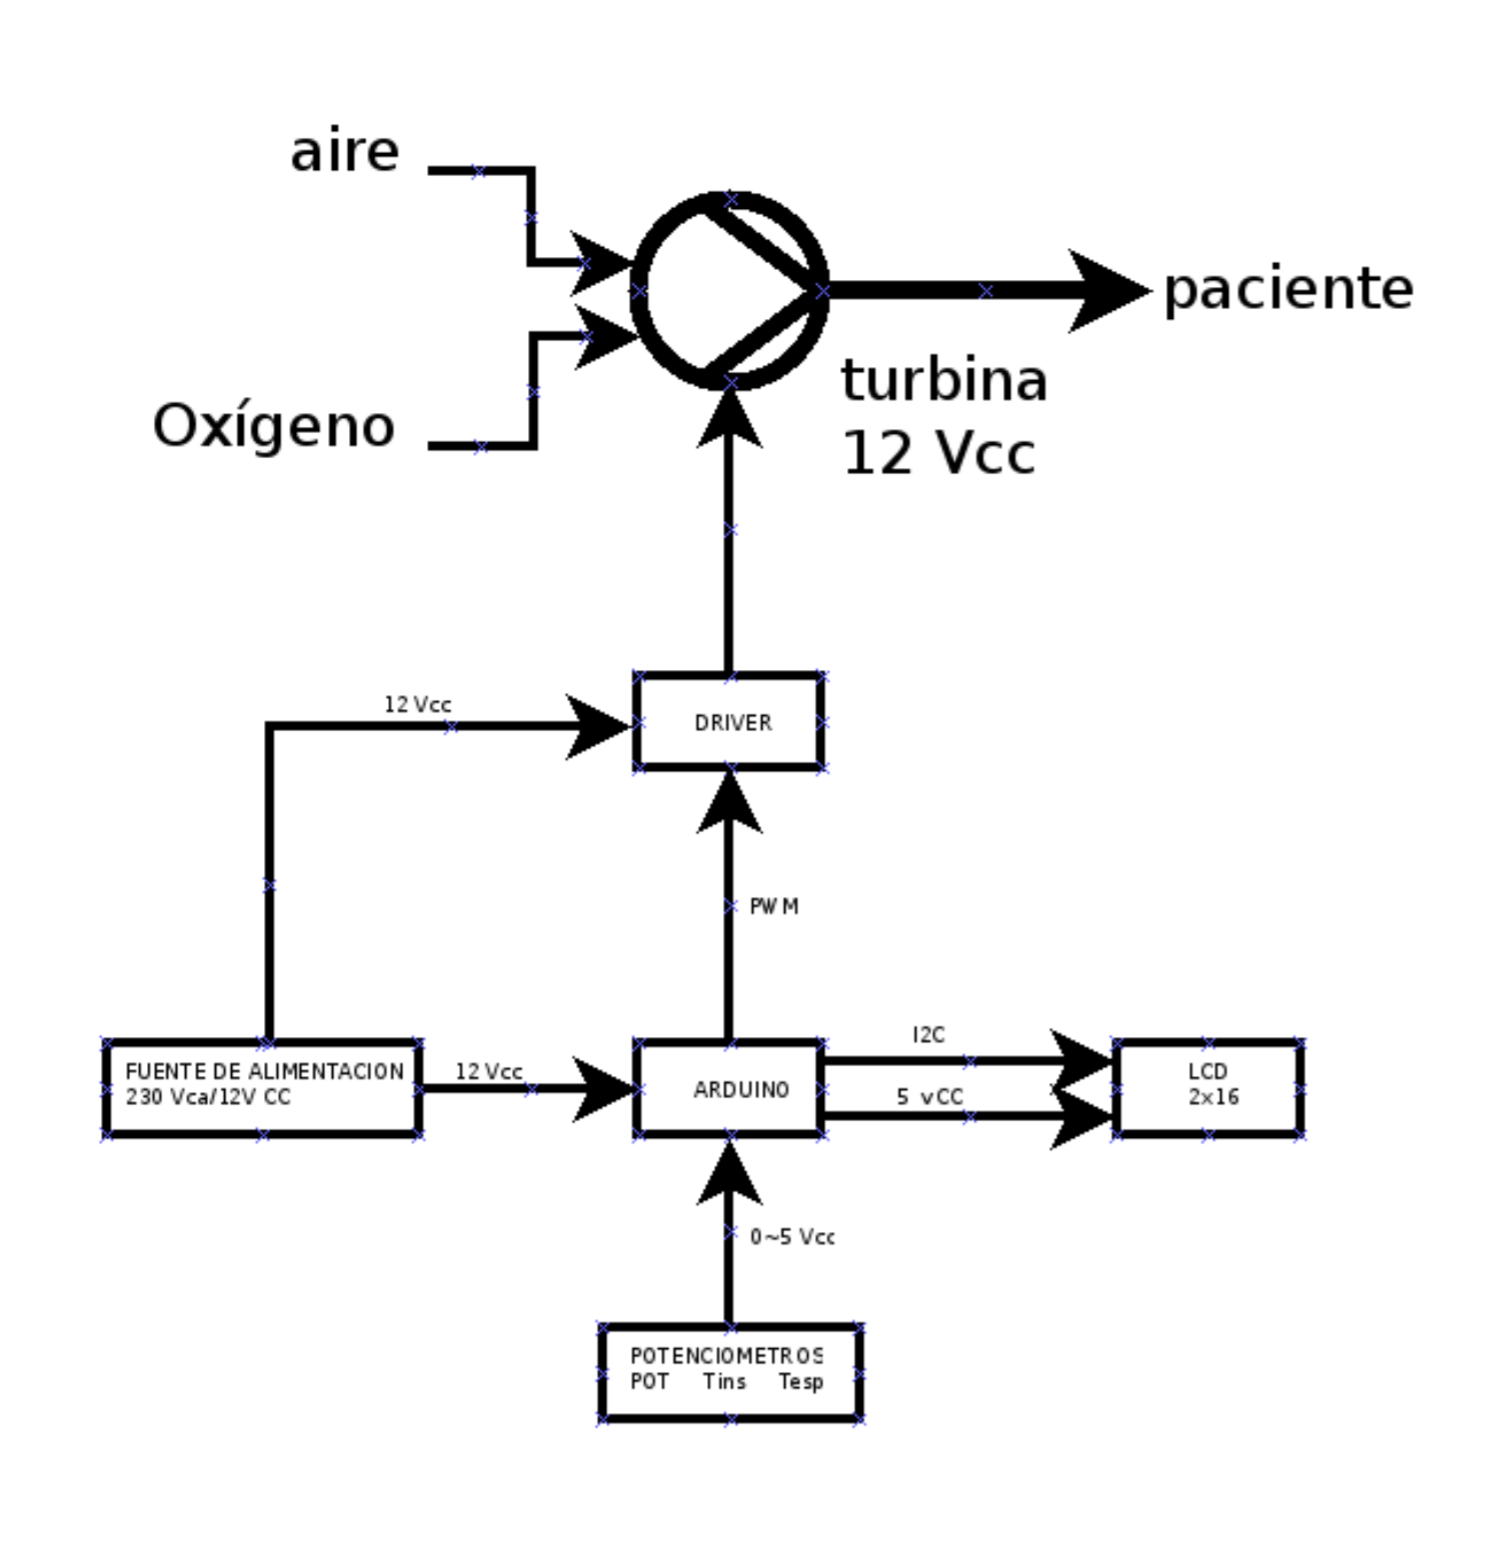
\includegraphics[width=0.4\textwidth]{Img/Bloques.PNG}
        \caption{Esquema de bloques}
    \end{figure}
    El respirador está compuesto por una turbina de aire, una tarjeta electrónica una fuente de alimentación y una caja de plástico.\\
    
    La turbina impulsora recoge aire (medicinal o atmosférico) y Oxígeno y lo lleva hasta el paciente con el ritmo y presión que determine el personal sanitario. Esa turbina está alimentada desde una placa electrónica que contiene el sistema de control (microcontrolador) y la pantalla. Los elementos de mando son tres potenciómetros situados en la tapa frontal (transparente) y conectados a la placa electrónica por cables. Una fuente de 12 \Vcc alimenta a la electrónica y a través de esta, a la turbina. El equipo puede ser alimentado por la batería de 12 \Vcc de una ambulancia. Por último, una caja de plástico con el frontal transparente constituye la envolvente eléctrica que dota de aislamiento al conjunto.
    
    Toda la maniobra y los valores de los parámetros y los valores límite de las variables están definidos por software.
    \begin{figure}
        \centering
        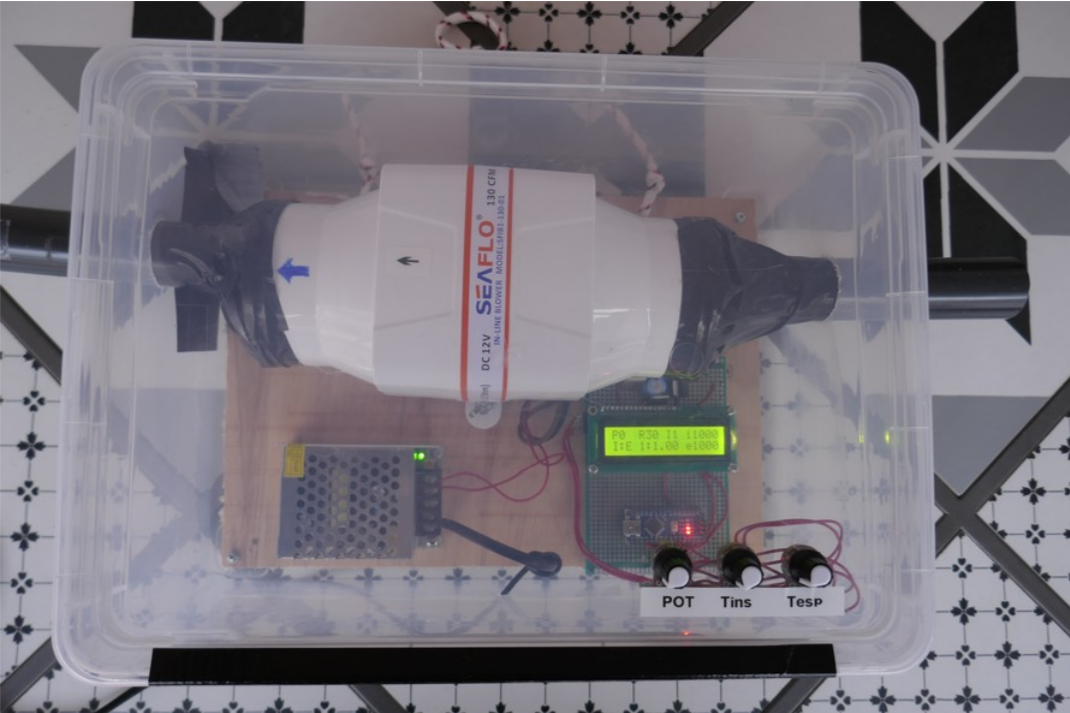
\includegraphics[width=0.4\textwidth]{Img/prototipo-1.PNG}
        \caption{Primer prototipo}
    \end{figure}
    
\subsection{Turbina}
    El soplador con motor eléctrico de 12 \Vcc o de 24 \Vcc está controlado por un transistor de potencia con modulación por anchura de pulso. El usado en el prototipo procede del mercado náutico (es un ventilador de sentina).\\
    Debe ser capaz de soplar 600 ml (800 ml excepcionalmente) a una presión de hasta 70 cmH\textsubscript{2}0\\
    Si hiciera falta usar un ventilador de corriente alterna a 230\Vca, debería rediseñarse tanto el hardware como el software (puede hacerse muy rápidamente).
\subsection{Tarjeta Electrónica}
    La tarjeta electrónica incorpora los siguientes elementos:
    \begin{itemize}
        \item Estabilizador de tensión
        \item Pantalla
        \item Ordenador
        \item Amplificador de salida al motor
    \end{itemize}
    El estabilizador de tensión tiene por objeto alimentar a 5 \Vcc a todos los elementos electrónicos activos. Está compuesto por un regulador integrado tipo \textit{7805} en caja \textit{TO220} sin radiador, con condensadores de filtro en la entrada y en la salida.\\

    La pantalla es del tipo LCD retroiluminada de dos filas de 16 caracteres, conectada al ordenador mediante un bus serie tipo \textit{I2C}.\\
    
    El ordenador es un modelo \textit{Arduino Nano} construido desde un microcontrolador ATMTEL \textit{ATmega328}. El     programa está desarrollado en el entorno \textit{Arduino} y se carga en memoria flash del ordenador por el interface USB. Se puede conseguir fácilmente en el mercado y es muy barato (desde 3€).\\
    
    El amplificador de salida del motor está constituido por un transistor de media potencia NPN en montaje Darlington tipo \textit{TIP120} y está diseñado para poder usar transistores FET-MOS encapsulados en el mismo tipo de caja (TO220), como el \textit{IRF3710}.
    
\subsection{Potenciómetros}
    Tres potenciómetros lineales montados sobre un pequeño circuito impreso constituyen los elementos de control sobre potencia máxima de la turbina, tiempo de inspiración y tiempo de espiración. Los tres están montados sobre la tapa frontal para hacerlos accesibles.\\
    Los valores límite máximo y mínimo de cada potenciómetro están definidos por software, así como las propias magnitudes que controlan, con lo que pueden modificarse fácilmente.
\subsection{Fuente de alimentación}
    La fuente de alimentación es un modelo disponible en todos los comercios especializados. Las características de tensión e intensidad vienen dadas por los requerimientos de la turbina, 12Vcc/2.5A. Por eso la fuente escogida es de 12Vcc/5A.
\subsection{Caja}
    Todo el conjunto se monta sobre una placa de montaje que a su vez se atornilla sobre el fondo de la caja. Esta debe proveer, no solo la robustez estructural del conjunto, sino también la protección mecánica y eléctrica necesaria en un entorno hospitalario. De ser capaz de ser limpiada y desinfectada en funcionamiento.\\
    Los ejemplares de producción final serán envolventes plásticas comerciales de las característica adecuadas con tapa transparente.